\documentclass[conference]{IEEEtran}

\usepackage[T1]{fontenc}
\usepackage[utf8]{inputenc}
\usepackage{cite}
\usepackage{amsmath,amssymb}
\usepackage{graphicx}
\usepackage{booktabs}
\usepackage{array}
\usepackage{url}

\title{Evidence-Constrained Neuro-Symbolic Ontology Repair for Semantic Drift in Versioned Normative Documents}

\author{\IEEEauthorblockN{Anonymous Authors}
\IEEEauthorblockA{Anonymous Affiliation\\
Email: anonymous@example.com}}

\begin{document}
\bstctlcite{IEEEexample:BSTcontrol}
\maketitle

\begin{abstract}
Versioned normative documents continuously revise definitions, obligations, exceptions, scopes, and effective conditions. Ontologies built from earlier document versions may therefore remain logically consistent while containing assertions that are no longer semantically supported by the current evidence. This paper presents ECR-Repair, an evidence-constrained neuro-symbolic framework for finite-candidate ontology repair under semantic drift. The central design is a Semantic Intermediate Representation (Semantic IR) that acts as a neural-symbolic interface between natural-language normative evidence and symbolic OWL/RDF repair decisions. Large language models are used to interpret evidence and, when needed, verify candidate entailment, but candidate content is isolated from semantic extraction so that repair is not reduced to an ``Evidence + Candidate $\rightarrow$ LLM $\rightarrow$ Answer'' prompt. Symbolic components perform typed semantic normalization, constraint-aware candidate ranking, selective gating, and formal validation through OWL consistency, RDF graph-delta checking, and competency-question regression. On an RFC-based benchmark containing 264 repair events and 1320 runs across three semantic drift types, ECR-Repair achieves 99.62\% closure accuracy and 99.24\% strict event success, outperforming both a direct LLM baseline and a base Semantic IR pipeline. The results show that reliable ontology repair for evolving normative sources requires not only language-model interpretation, but also explicit evidence constraints, candidate-content isolation, and formal symbolic closure.
\end{abstract}

\begin{IEEEkeywords}
ontology repair, semantic drift, neuro-symbolic reasoning, Semantic IR, large language models, OWL, RDF, evidence grounding
\end{IEEEkeywords}

\section{Introduction}

Ontologies are widely used to represent regulatory requirements, protocol standards, domain policies, and other normative knowledge. In these settings, correctness depends not only on whether an ontology is internally consistent, but also on whether its assertions are still supported by the current version of the underlying normative documents. Normative documents are not static. A new version may supersede an earlier specification; an exception may override a general rule; a qualifier may change the scope of multiple statements; or an effective date may alter which condition is currently applicable. These changes can create semantic drift between an ontology and its evidence source.

The key difficulty is that semantic drift is not the same as syntactic invalidity or logical inconsistency. Existing ontology repair methods mainly detect logical inconsistency, while semantically outdated but logically valid assertions remain difficult to identify. An outdated ontology assertion may still be well formed, may satisfy the declared ontology vocabulary, and may pass a reasoner consistency check. For example, an assertion saying that a standard version $X$ is current may remain logically consistent after version $Y$ supersedes $X$, because the ontology contains no contradiction unless the supersession semantics have been represented and checked. Thus, logical consistency $\not\Rightarrow$ semantic correctness. Textual differencing alone is also insufficient, since versioned normative documents often express changes through dispersed temporal anchors, exception clauses, and cross-sentence scope relations.

Large language models (LLMs) offer a natural mechanism for interpreting such normative language. However, directly asking an LLM to repair an ontology introduces three practical risks. First, the model may hallucinate an unsupported repair, especially when the evidence is incomplete or linguistically complex \cite{ji2023hallucination}. Second, a direct prompt may not expose a traceable path from evidence to ontology edit. Third, even a plausible natural-language answer may not produce an OWL/RDF patch that preserves declared graph effects and downstream competency-question behavior. These limitations are particularly problematic when the ontology is used as an operational representation of normative constraints.

This paper proposes ECR-Repair, an evidence-constrained neuro-symbolic ontology repair framework. Instead of treating repair as direct generation, ECR-Repair decomposes the task into five roles:
\[
\begin{gathered}
\text{Normative Evidence}
\rightarrow
\text{Semantic IR}
\rightarrow
\text{Symbolic Decision}\\
\rightarrow
\text{Fallback Verification}
\rightarrow
\text{OWL/RDF Validation}.
\end{gathered}
\]
The Semantic Intermediate Representation (Semantic IR) is the central neural-symbolic interface: it converts evidence into typed semantic fields before candidates are ranked. For example, if an old ontology states that specification $X$ is current while the current normative evidence says that specification $Y$ updates $X$ and governs the target requirement, Semantic IR records the entities $X$ and $Y$, the update relation, the current/effective role of $Y$, the obsolete or historical role of $X$, and the supporting evidence span. Candidate ranking then prefers the repair that replaces $X$ with $Y$ and rejects candidates that retain $X$ or reverse the update direction.

This workflow explicitly separates evidence interpretation from candidate selection. The semantic interpretation module does not read candidate values, candidate operations, candidate identifiers, candidate scores, or top-$k$ identities. Only after a candidate-blind Semantic IR has been fixed does the system reveal the finite candidate set. This avoids the shortcut
\[
\text{Evidence + Candidate} \rightarrow \text{LLM} \rightarrow \text{Answer}
\]
and instead follows
\[
\text{Evidence} \rightarrow \text{Semantic IR} \rightarrow \text{Candidate Ranking}.
\]
If ranking remains ambiguous, a fallback verifier may evaluate candidates independently, but only in the candidate-aware decision layer and under fixed abstention rules.

This conference version focuses on the method and an initial empirical validation. It frames the task as evidence-relative semantic repair with a provided event, evidence window, and finite candidate set; automatic drift discovery, open-corpus retrieval, and open-ended candidate generation are outside scope.

The contributions are:
\begin{itemize}
    \item We propose ECR-Repair, an evidence-constrained neuro-symbolic ontology repair framework for semantic drift in versioned normative documents.
    \item We introduce Semantic IR as an explicit interface between LLM-based evidence interpretation and symbolic reasoning, together with a candidate-content isolation protocol that prevents candidate leakage before ranking.
    \item We define formal closure validation for selected OWL/RDF repairs and evaluate the method on 264 RFC-based repair events and 1320 runs, showing substantial gains over direct LLM and base Semantic IR baselines.
\end{itemize}

\section{Related Work}

\subsection{Ontology Evolution and Repair}

Ontology evolution and repair study how changes in a knowledge source or conceptualization should be propagated while maintaining usability, consistency, and constraint satisfaction. Recent SHACL and constraint-repair work provides one setting in which RDF graph violations are detected and repaired against explicit shapes \cite{ahmetaj2022shacl,ahmetaj2025shacl}. These approaches are essential for structural and logical quality, but they do not by themselves guarantee that an assertion remains supported by a revised normative document.

Our setting is narrower and different. We assume that a potential local repair event has been identified and that a finite set of executable repair candidates is available. The task is to select the candidate whose semantics are supported by current evidence and then validate the resulting OWL/RDF patch. This places semantic interpretation before formal closure: formal checks can reject malformed, inconsistent, or undeclared edits, but they cannot determine whether a formally valid candidate is the one best supported by the current normative evidence.

\subsection{LLM-Based Ontology Engineering}

Recent work has explored LLMs for ontology learning, requirements elicitation, competency-question generation, ontology drafting, and ontology testing \cite{giglou2024llms4ol,lippolis2025ontologygeneration,zhang2025ontochat,fathallah2025neongpt}. LLMs can reduce the cost of moving from textual requirements to structured knowledge, and broader work on LLMs and knowledge graphs suggests many opportunities for combining language models with symbolic graph representations \cite{pan2024llmkg}. At the same time, LLM outputs may be hallucinated, structurally unstable, or difficult to validate \cite{ji2023hallucination}.

ECR-Repair therefore adopts a conservative use of LLMs. The model does not directly rewrite the ontology. It first interprets evidence into Semantic IR, and only a later symbolic decision layer maps that IR to candidate edits. When candidate ambiguity remains, LLM-based verification is used as a fallback entailment check, not as an unconstrained repair generator.

\subsection{Neuro-Symbolic Reasoning}

Neuro-symbolic AI combines neural models' pattern-recognition and language-understanding strengths with symbolic systems' explicit structure, constraints, and reasoning \cite{yu2023neurosymbolic}. Knowledge graphs provide a natural symbolic substrate for such integration, since they encode entities, relations, constraints, and graph structure in machine-checkable form \cite{hogan2021knowledgegraphs}. Retrieval-augmented generation further shows that language models can benefit from external evidence when generation is grounded in retrieved or selected context \cite{gao2024rag,asai2023selfrag}.

ECR-Repair follows this general direction but applies it to ontology repair under versioned normative evidence. The neural layer converts evidence into a structured semantic representation. The symbolic layer enforces type constraints, candidate admissibility, graph-delta consistency, and competency-question regression. Selective prediction also informs the design: when the available evidence or ranking signal is insufficient, the system should abstain rather than force a repair \cite{gu2023selective}.

\section{Problem Formulation}

Let $O$ be a source ontology that may contain an assertion no longer supported by current normative evidence. Let $D$ be a collection of versioned normative documents, and let $C=\{c_1,\ldots,c_k\}$ be a finite candidate set for a localized repair event. Each candidate $c_i$ contains a display value and a formal OWL/RDF edit operation. The output is either a selected repair candidate $c^\ast$ or \textsc{Abstain}.

The input is therefore:
\[
(O,D,C),
\]
where the event metadata specify the target subject, predicate, semantic type, and evidence window. The output is:
\[
c^\ast \in C \cup \{\textsc{Abstain}\}.
\]
A selected candidate is accepted only if it is supported by the current evidence and its OWL/RDF patch passes formal validation. The private oracle, used only for evaluation, is excluded from all model prompts and decision inputs.

This paper studies evidence-relative semantic repair rather than automatic drift discovery. The task assumes that a potential drift location, a relevant evidence window, and a finite candidate set have already been provided. The method is therefore not evaluated as an end-to-end system for scanning a complete corpus, retrieving all evidence, generating candidate patches, or proving historical drift across all document versions.

The distinction matters because semantic drift is defined relative to evidence support. Let $\mathrm{Support}(a,D_t)$ denote whether assertion $a$ is supported by evidence at time or version $t$. The present task uses the current-evidence condition: the old assertion is not supported by the current evidence window, and one candidate repair is supported by it.

\section{ECR-Repair Framework}

\subsection{Overview}

Fig.~\ref{fig:framework} shows the overall architecture. ECR-Repair is organized as a modular neuro-symbolic pipeline. Normative evidence is first filtered and interpreted into Semantic IR. The fixed IR is then used by a symbolic decision layer to rank candidates under semantic and structural constraints. If ranking is ambiguous, a fallback verifier evaluates candidate entailment under fixed rules. Finally, the selected repair is materialized as an OWL/RDF patch and validated through formal checks.

\begin{figure*}[t]
    \centering
    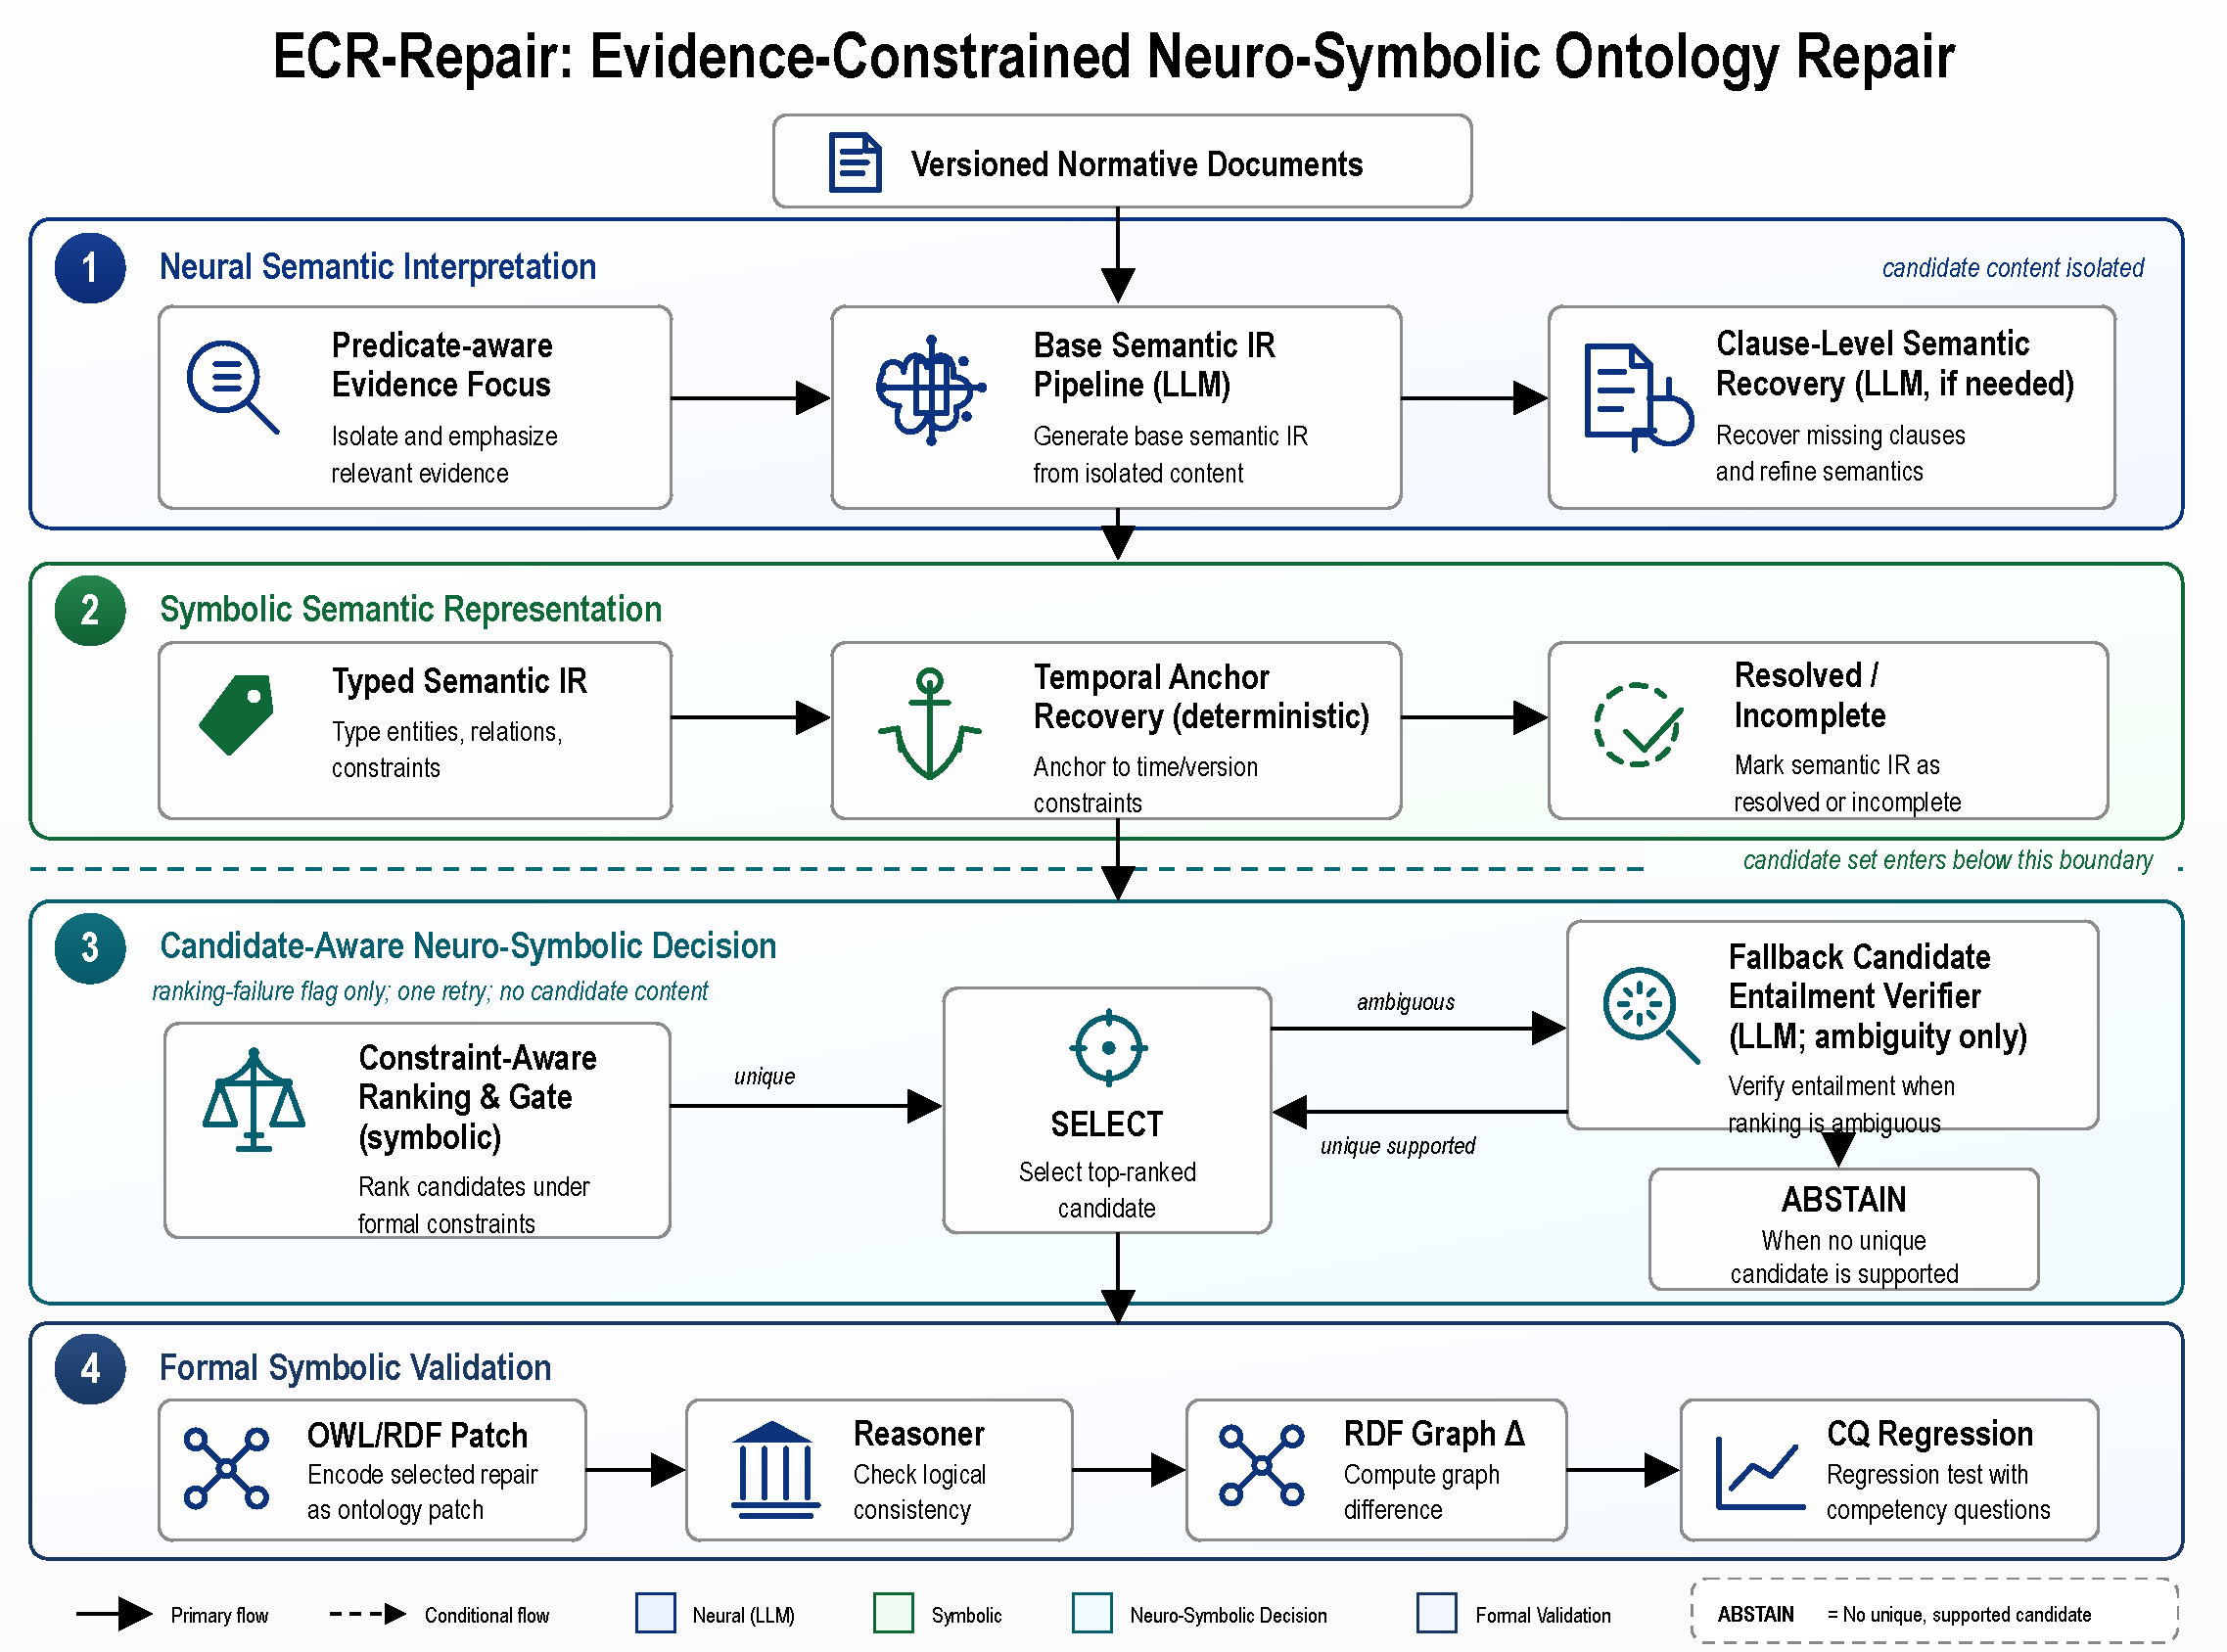
\includegraphics[width=\textwidth]{figures/neurosymbolic_framework.pdf}
    \caption{Overall evidence-constrained neuro-symbolic architecture of ECR-Repair. Semantic IR is the neural-symbolic interface; candidate content becomes visible only after evidence interpretation has been fixed.}
    \label{fig:framework}
\end{figure*}

The framework follows five stages:
\begin{enumerate}
    \item \textbf{Normative Evidence.} The system receives a versioned normative evidence window and public event metadata.
    \item \textbf{Semantic IR.} An LLM-supported interpretation module converts evidence into typed semantic fields without access to candidate content.
    \item \textbf{Symbolic Decision.} A deterministic scorer ranks candidate operations against the fixed IR and applies selective gates.
    \item \textbf{Fallback Verification.} If ranking cannot identify a unique admissible candidate, a candidate-level entailment verifier evaluates candidates independently.
    \item \textbf{OWL/RDF Validation.} The selected edit is materialized, checked for OWL consistency, compared through RDF graph delta, and tested by competency-question regression.
\end{enumerate}

\subsection{Semantic IR as Neural-Symbolic Interface}

Semantic IR is the central interface contract between language interpretation and symbolic repair. It is not a new name for prompt engineering, a free-form rationale, or a candidate answer; it is a typed representation of what the evidence says about the target assertion before any candidate content is visible.

For each repair event, Semantic IR records:
\begin{itemize}
    \item \textbf{Entity}: the subject, object, version, standard, condition, or other normative entity involved in the assertion;
    \item \textbf{Relation}: the relevant predicate, rule relation, exception relation, version relation, or scope relation;
    \item \textbf{Temporal information}: current version, superseded version, effective date, publication date, reference date, or unresolved temporal anchor;
    \item \textbf{Scope}: the statement or set of statements governed by a qualifier, exception, condition, or cross-sentence modifier;
    \item \textbf{Constraint}: type restrictions, rule priority, negation, numeric/date constraints, and admissibility conditions;
    \item \textbf{Evidence}: explicit spans or document fragments supporting the extracted fields.
\end{itemize}

The representation is type specific. Temporal-Version events encode current, superseded, effective, publication, and reference roles. General Rule-Exception events encode a general rule, exception trigger, exception result, and priority. Cross-Sentence Scope events encode the qualified statement, qualifier, scope target, and attachment relation. If required fields cannot be supported by evidence, the IR is marked incomplete and the system abstains or invokes a candidate-blind recovery step.

This structure is what makes the method neuro-symbolic: the neural component interprets complex normative language, while the symbolic component receives a typed object whose fields can be inspected, constrained, and mapped to formal ontology edits.

\subsection{Candidate-Content Isolation}

A central design constraint is candidate-content isolation. During evidence interpretation, the model sees the evidence window and public event metadata, but not candidate values, candidate operations, candidate identifiers, candidate scores, or the private oracle. Candidate information enters only after Semantic IR has been produced and normalized.

This avoids an important leakage path. If a prompt contains both evidence and candidate text, an LLM may choose the candidate whose wording best matches the evidence without constructing an independent semantic representation. Such a system can appear accurate on finite-choice benchmarks while failing to provide a stable evidence-to-ontology interface. ECR-Repair instead fixes the semantic interpretation first:
\[
\text{Evidence}
\rightarrow
\text{Semantic IR}
\rightarrow
\text{Candidate Ranking}.
\]
Only a content-free failure signal may flow backward. For General Rule-Exception and Cross-Sentence Scope events, if candidate ranking fails to produce a unique admissible candidate, the semantic recovery module may receive the Boolean flag \texttt{ranking\_failed=true} and perform at most one additional candidate-blind recovery pass. It does not receive the leading candidate, the scores, the candidate values, or any candidate-derived semantics.

\subsection{Symbolic Decision and Constraint Scoring}

After Semantic IR is fixed, ECR-Repair reveals the finite candidate set and scores each candidate against the evidence-grounded representation. The decision layer is symbolic in the sense that it uses typed fields, deterministic constraints, and explicit gate conditions rather than free-form generation.

For exposition, the decision objective can be summarized as semantic match plus constraint satisfaction minus conflicts. In the implementation used for the reported experiments, the lexical-constraint component is instantiated as:
\[
\begin{aligned}
s(c_i)=&0.30s_f+0.26s_t+0.20\max(s_c,s_n)\\
&+0.12s_n+0.08s_c+0.04s_e+b_{\mathrm{sem}}-p_{\mathrm{neg}} .
\end{aligned}
\]
$s_f$, $s_t$, $s_c$, $s_n$, and $s_e$ measure source-family, lexical, code, numeric, and exact-value agreement with Semantic IR. $b_{\mathrm{sem}}$ rewards current, integrated, or superseded markers under version relations, while $p_{\mathrm{neg}}$ penalizes obsolete, absent, negated, or reversed markers. These weights are fixed heuristic design choices from pilot implementation, not parameters fitted on the final benchmark; their ordering reflects the priority of source-family and lexical agreement over exact-value matches and small semantic bonuses. Type-specific constraint reranking then checks role, value, direction, exception priority, and scope attachment constraints. The reported experiments use frozen gates: the default minimum score is 0.30, the General Rule-Exception and Cross-Sentence Scope threshold is 0.24, the minimum margin is 0.00, and Temporal-Version events permit a unique non-contradicted top candidate under the temporal gate.

The gate accepts a ranked candidate only if it is unique and admissible. A candidate may be rejected because the Semantic IR is incomplete, its score is below the threshold, another candidate ties under the relevant constraints, or an explicit conflict is detected. The gate is selective: abstention is a valid outcome and is preferred to an unsupported ontology edit.

\subsection{Fallback Verification}

The fallback verifier is invoked only when symbolic ranking remains ambiguous. Unlike the initial Semantic IR stage, the verifier is candidate aware. However, it evaluates each candidate independently rather than asking the model to compare all candidates in one prompt. For each candidate, the verifier determines whether the candidate operation is \texttt{supported}, \texttt{contradicted}, \texttt{unrelated}, or \texttt{underspecified} with respect to the fixed evidence and Semantic IR.

A candidate can proceed only when exactly one candidate is supported with sufficient confidence. Multiple supported candidates, no supported candidates, low confidence, contradiction, or underspecification all lead to \textsc{Abstain}. This preserves the division of responsibility: the verifier may resolve residual semantic ambiguity, but it does not replace the symbolic gate or formal closure.

\subsection{Formal Validation}

The final stage validates the selected repair as an OWL/RDF operation under graph-based knowledge representation, RDF validation, and OWL reasoning practice \cite{hogan2021knowledgegraphs,pareti2021shaclreview,heist2021caligraph}. Each candidate has a declared edit set:
\[
\Delta_{c_i}=(\Delta^-_{c_i},\Delta^+_{c_i}),
\]
where $\Delta^-_{c_i}$ contains target deletions and $\Delta^+_{c_i}$ contains target additions. Applying the candidate to $O$ yields a repaired ontology $O'$. ECR-Repair accepts the patch only if all formal validation checks pass:
\begin{itemize}
    \item \textbf{OWL consistency}: the repaired ontology is materialized and checked for logical consistency under the configured reasoner;
    \item \textbf{RDF graph delta}: the realized graph difference matches the candidate-declared additions and deletions, with no undeclared side effects;
    \item \textbf{CQ regression}: frozen competency-question or repair-regression checks continue to return the expected results after the patch.
\end{itemize}

These checks provide formal safety, but they do not replace semantic selection. A semantically wrong candidate may still be logically consistent. Therefore, ECR-Repair treats formal validation as a necessary but not sufficient condition for semantic repair.

\section{Experiments}

\subsection{Dataset}

To the best of our knowledge, there is no off-the-shelf benchmark that directly evaluates evidence-relative ontology repair for semantic drift in versioned normative documents. Existing resources for ontology repair, knowledge-graph completion, or document-grounded question answering do not jointly provide evolving normative evidence, localized ontology assertions, executable OWL/RDF repair candidates, and formal closure checks. We therefore construct an RFC-based finite-candidate benchmark for this study. Each event provides a localized ontology assertion, current normative evidence, a semantic type, and three executable repair candidates. The candidate set contains one manually reviewed evidence-supported repair and two distractors designed to be executable but semantically wrong, such as retaining an obsolete version, reversing a supersession relation, mismatching an exception condition, or attaching a scope qualifier to the wrong statement.

As a concrete example, a Temporal-Version event may include Candidate A: delete \texttt{(:s :currentSpec :X)} and add \texttt{(:s :currentSpec :Y)}; Candidate B: retain or reassert \texttt{(:s :currentSpec :X)}; and Candidate C: reverse the update direction with \texttt{(:X :supersedes :Y)}. All three are executable graph edits, but only Candidate A is supported when the evidence states that $Y$ updates $X$ and governs the current requirement. Table~\ref{tab:dataset} summarizes the benchmark.

\begin{table}[t]
\centering
\caption{Dataset summary}
\label{tab:dataset}
\begin{tabular}{lr}
\toprule
Item & Value \\
\midrule
Events & 264 \\
Runs & 1320 \\
Types & 3 \\
Candidates/event & 3 \\
\bottomrule
\end{tabular}
\end{table}

The three event types correspond to the main semantic drift patterns addressed by the framework: Temporal-Version, General Rule-Exception, and Cross-Sentence Scope. The evaluation unit is a local repair event, not the size of the full ontology. The experiment therefore measures whether a method can select and validate the correct local OWL/RDF patch once a potential drift event and its evidence window have been provided.

\subsection{Compared Methods}

We compare three methods. \textbf{Direct LLM} receives evidence and candidate content and directly selects among candidates. It represents the natural prompting baseline, but it does not enforce candidate-content isolation or formal closure. \textbf{Base Semantic IR} uses evidence-grounded Semantic IR and symbolic repair logic, but does not include the full ECR-Repair recovery and fallback verification design. \textbf{ECR-Repair} uses the complete pipeline described in Section IV, including candidate-content-isolated Semantic IR, constraint-aware symbolic decision, fallback verification, and OWL/RDF validation.

The goal of these baselines is not to compare token cost or latency. Direct LLM and ECR-Repair have different call structures because ECR-Repair separates semantic interpretation, ranking, verification, and formal closure. The comparison instead asks whether explicit neuro-symbolic structure improves repair reliability over direct candidate selection and over the base Semantic IR pipeline.

\subsection{Metrics}

Closure accuracy is the percentage of runs in which the method selects the evidence-supported candidate and, for repair pipelines, the corresponding OWL/RDF repair passes formal validation. Strict success is the event-level success rate: an event is strictly successful only if the method succeeds across the repeated runs for that event. For Direct LLM, strict success is not reported because the baseline directly selects a candidate and does not execute the full formal closure pipeline; Table~\ref{tab:main_result} therefore uses closure accuracy as the common comparison metric.

\subsection{Main Result}

Table~\ref{tab:main_result} reports the main comparison. ECR-Repair achieves 99.62\% closure accuracy and 99.24\% strict success, improving substantially over both baselines. The Direct LLM baseline reaches 93.48\% under direct candidate exposure, showing that the task is not impossible for a language model. However, the remaining errors motivate a design that separates evidence interpretation from candidate choice and validates the final repair formally. The Base Semantic IR pipeline reaches 77.42\% closure accuracy and 73.86\% strict success, indicating that structured evidence interpretation alone is not enough; candidate-content isolation must be combined with constraint-aware ranking, selective gating, and fallback verification.

\begin{table}[t]
\centering
\caption{Main result on the conference benchmark}
\label{tab:main_result}
\begin{tabular}{lcc}
\toprule
Method & Closure Accuracy & Strict Success \\
\midrule
Direct LLM & 93.48\% & -- \\
Base Semantic IR & 77.42\% & 73.86\% \\
ECR-Repair & 99.62\% & 99.24\% \\
\bottomrule
\end{tabular}
\end{table}

\subsection{Error Analysis}

The remaining failures occur as abstentions rather than unsupported patches. A representative failure is a General Rule-Exception event in which the Semantic IR identifies the relevant rule and exception, but the verifier cannot isolate exactly one evidence-supported candidate under the fixed gate. Similar boundary cases arise when a qualifier can attach to more than one nearby statement. The residual risk is therefore underdetermined exception or scope resolution among executable candidates, not OWL materialization failure.

\section{Discussion}

The conference version evaluates repair decision quality after a potential event, evidence window, and finite candidate set are available; full-corpus drift discovery, evidence retrieval, and candidate generation are journal extensions. Formal validation remains necessary but not sufficient: OWL consistency, RDF graph-delta checking, and CQ regression catch unintended formal effects, but they cannot decide semantic support by themselves. ECR-Repair therefore restricts LLMs to evidence interpretation and residual entailment rather than unrestricted ontology editing. The benchmark uses manually reviewed candidates; a systematic inter-annotator agreement study is planned as part of a public dataset release to further strengthen benchmark reliability.

\section{Conclusion}

This paper presented ECR-Repair, an evidence-constrained neuro-symbolic framework for ontology repair under semantic drift in versioned normative documents. It uses Semantic IR as a neural-symbolic interface, isolates candidate content during semantic interpretation, ranks candidates through symbolic constraints, verifies ambiguity selectively, and validates selected patches through OWL consistency, RDF graph delta, and CQ regression. On 264 RFC-based repair events and 1320 runs, ECR-Repair reaches 99.62\% closure accuracy and 99.24\% strict event success, showing that reliable repair requires disciplined separation among evidence interpretation, symbolic decision, selective abstention, and formal closure.

\bibliographystyle{IEEEtran}
\bibliography{refs}

\end{document}
